\documentclass[11pt]{article}
\usepackage[margin=1.25in]{geometry}
\usepackage{setspace}
\usepackage{graphicx}
\usepackage{changepage}

% Changes section numbering from 1, 2, 3 to 1.0, 2.0, 3.0
\renewcommand*\thesection{\arabic{section}.0}
\renewcommand*\thesubsection{\arabic{section}.\arabic{subsection}}

\begin{document}

\title{PID Tuning Instructions for a Line-Following Robot}
\author{Rowan Walsh \& John Harvey \\ (30817118) (29240116)}
\date{\today}

\maketitle
\doublespacing

\section{Introduction}

Proper tuning of the PID algorithm used by a line-following robot is essential for efficient line-following and is a useful skill for Engineering Physics students during the ENPH 253 robot competition.  This set of PID-Tuning instructions is intended for the small line-following robots built in the ENPH 253 labs and the PID Line Following firmware written by Group 9.  Besides the robot, a charged LiPo battery and tape-course are needed.  Some of the components on the robot's microcontroller (the TINAH board) can get quite hot during normal operation, use caution and check for heat before touching components.  PID tuning involves changing the P gain (proportional gain), D gain (derivative gain), speed, and reflectance sensor threshold.

\section{PID Tuning Steps}

The steps taken when tuning a PID controlled line following robot are described below.

\begin{adjustwidth}{1cm}{}
\subsection{Setting up the TINAH Board}

	Start the TINAH board by connecting the LiPo battery and turning the power on using the switch shown in Figure 1. After several seconds, the TINAH board will turn on. The robot is ready once the TINAH board's LCD screen has turned on.
	
	\begin{figure}[h]
	\centering
		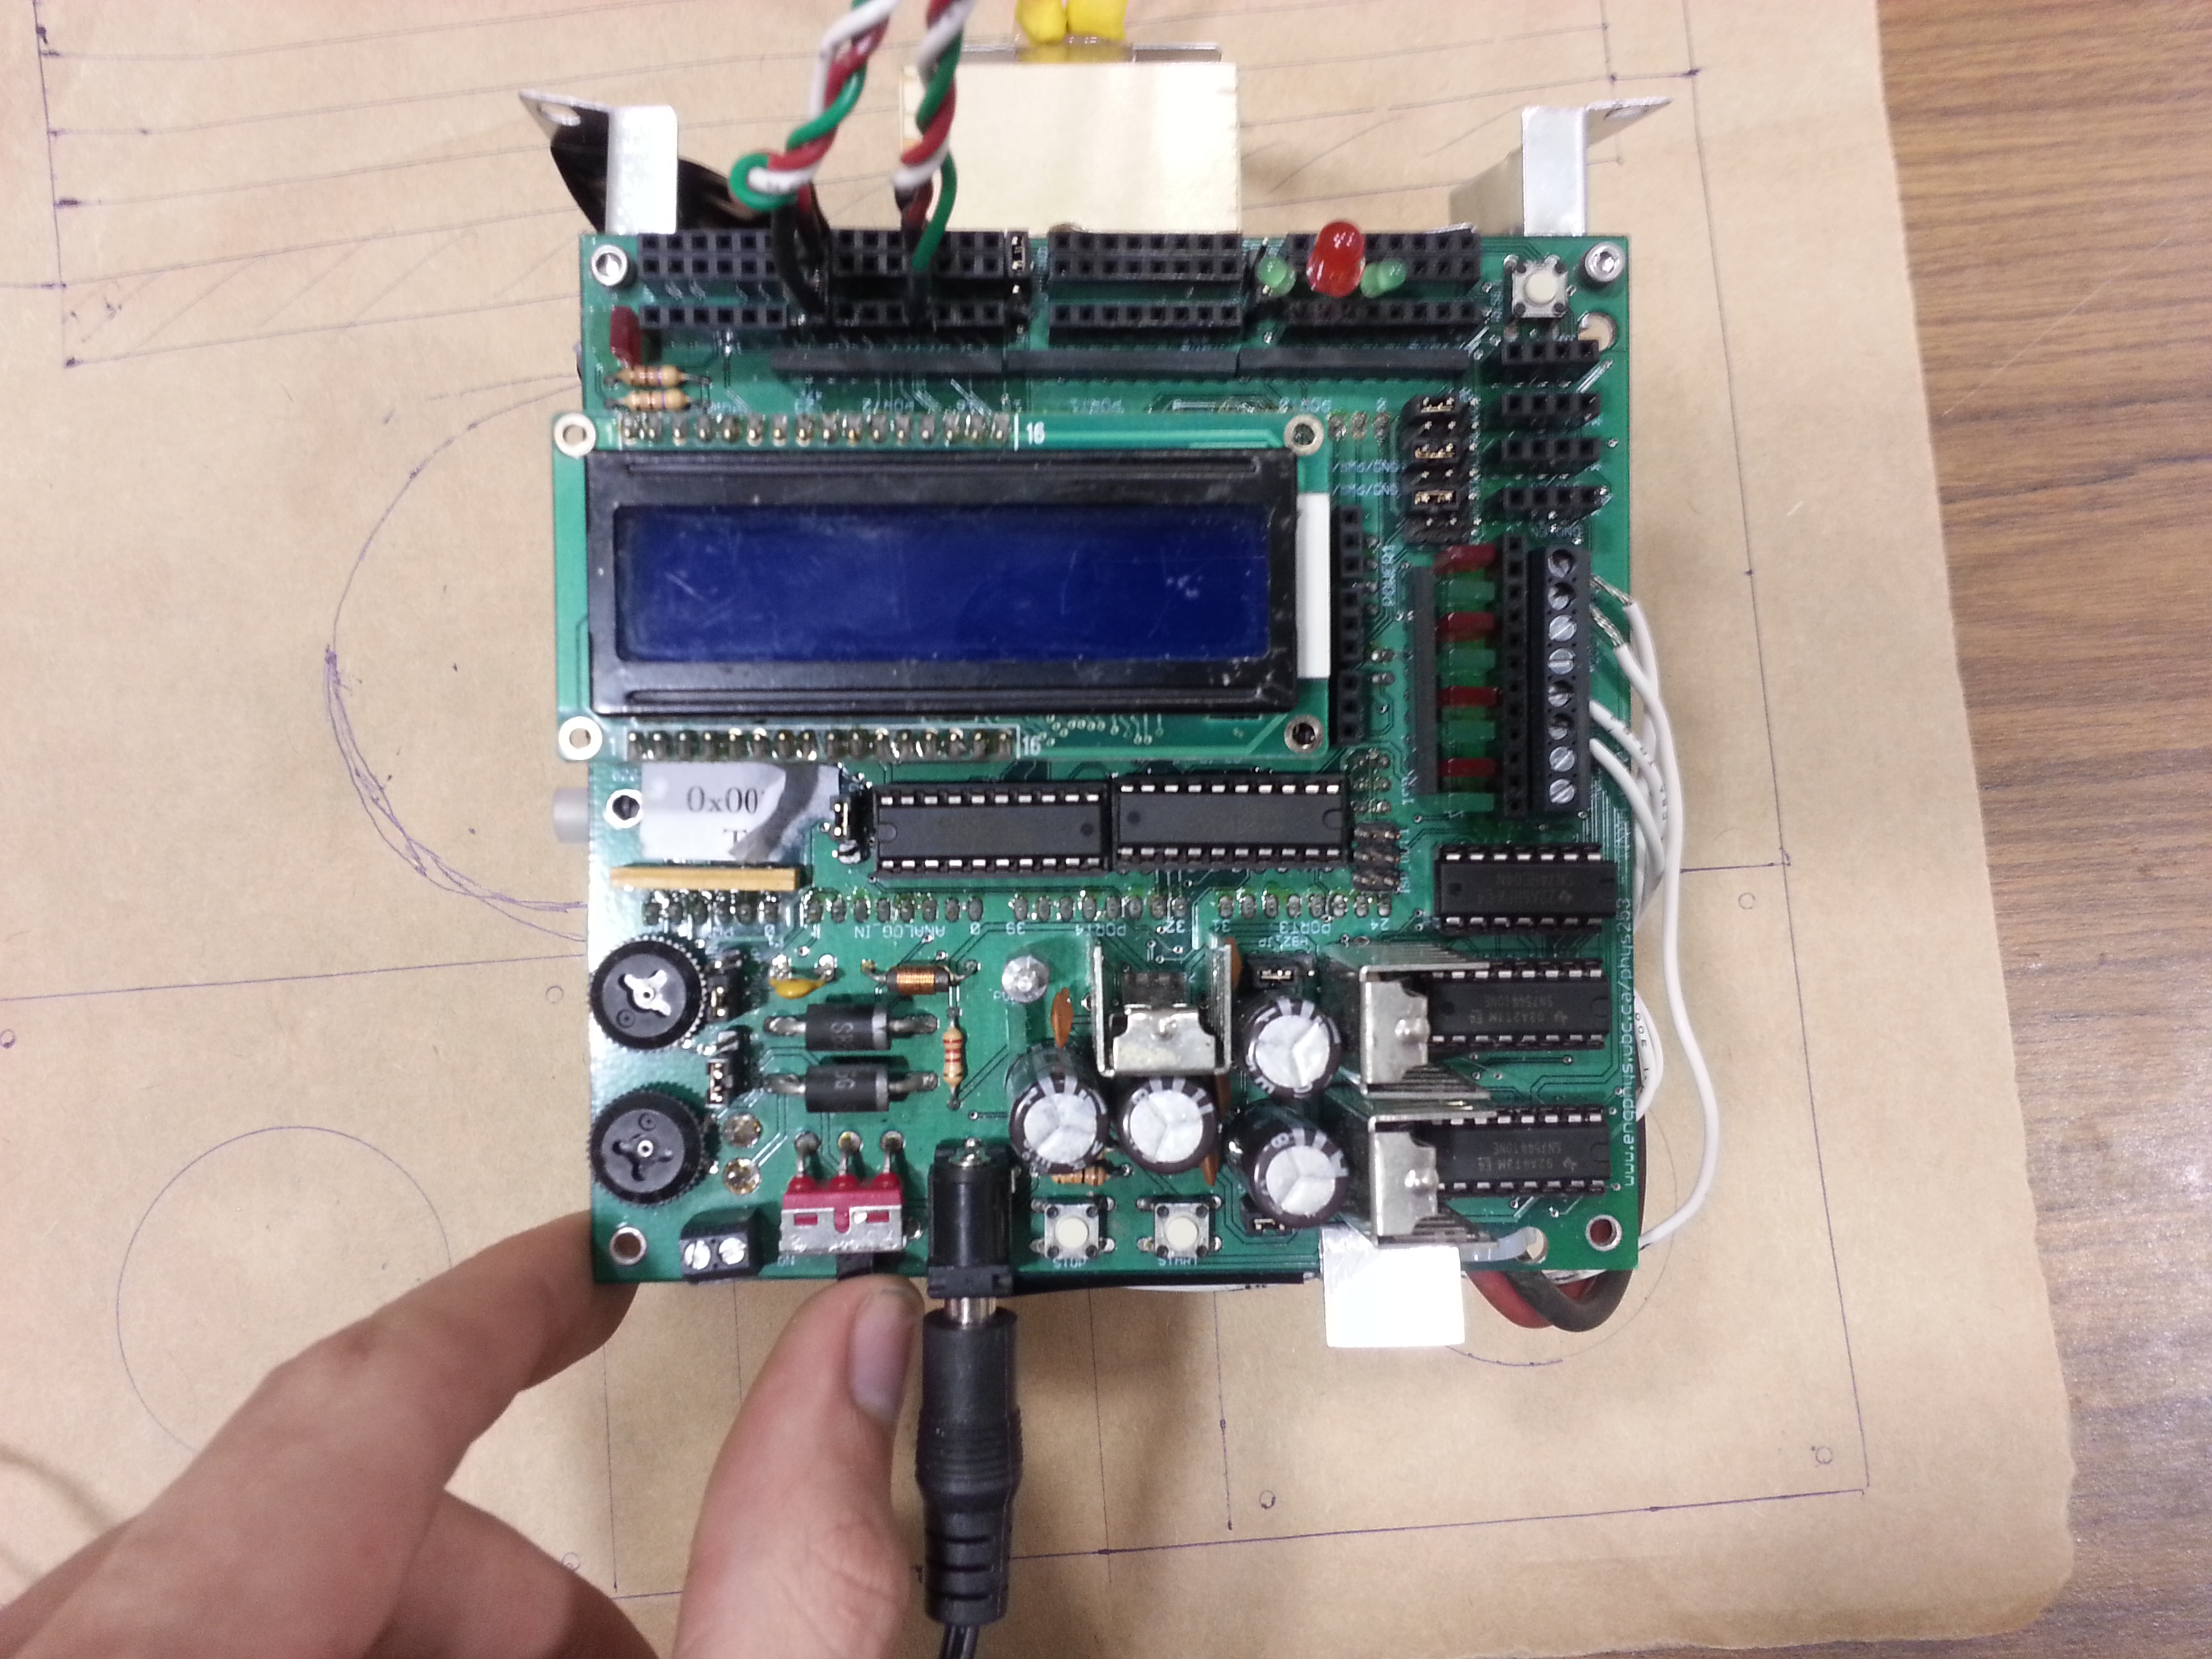
\includegraphics[width=0.7\textwidth]{Figures/power_switch.jpg}
		\caption{Toggling the TINAH board's ON/OFF switch.}
	\end{figure}

\subsection{Adjusting the Sensors}

Sensor placement is very important. The most accurate tape measurements occur when the sensors are placed very close to the ground, it is good practice to position the sensors no more than 3 mm away. The sensor location can be adjusted by bending the metal bracket that holds the sensors. The sensor bracket and IR sensors can be seen in Figure 2.  Be aware that changing the sensor positions will always require the Threshold parameter to be readjusted.
 
	\begin{figure}[h]
	\centering
		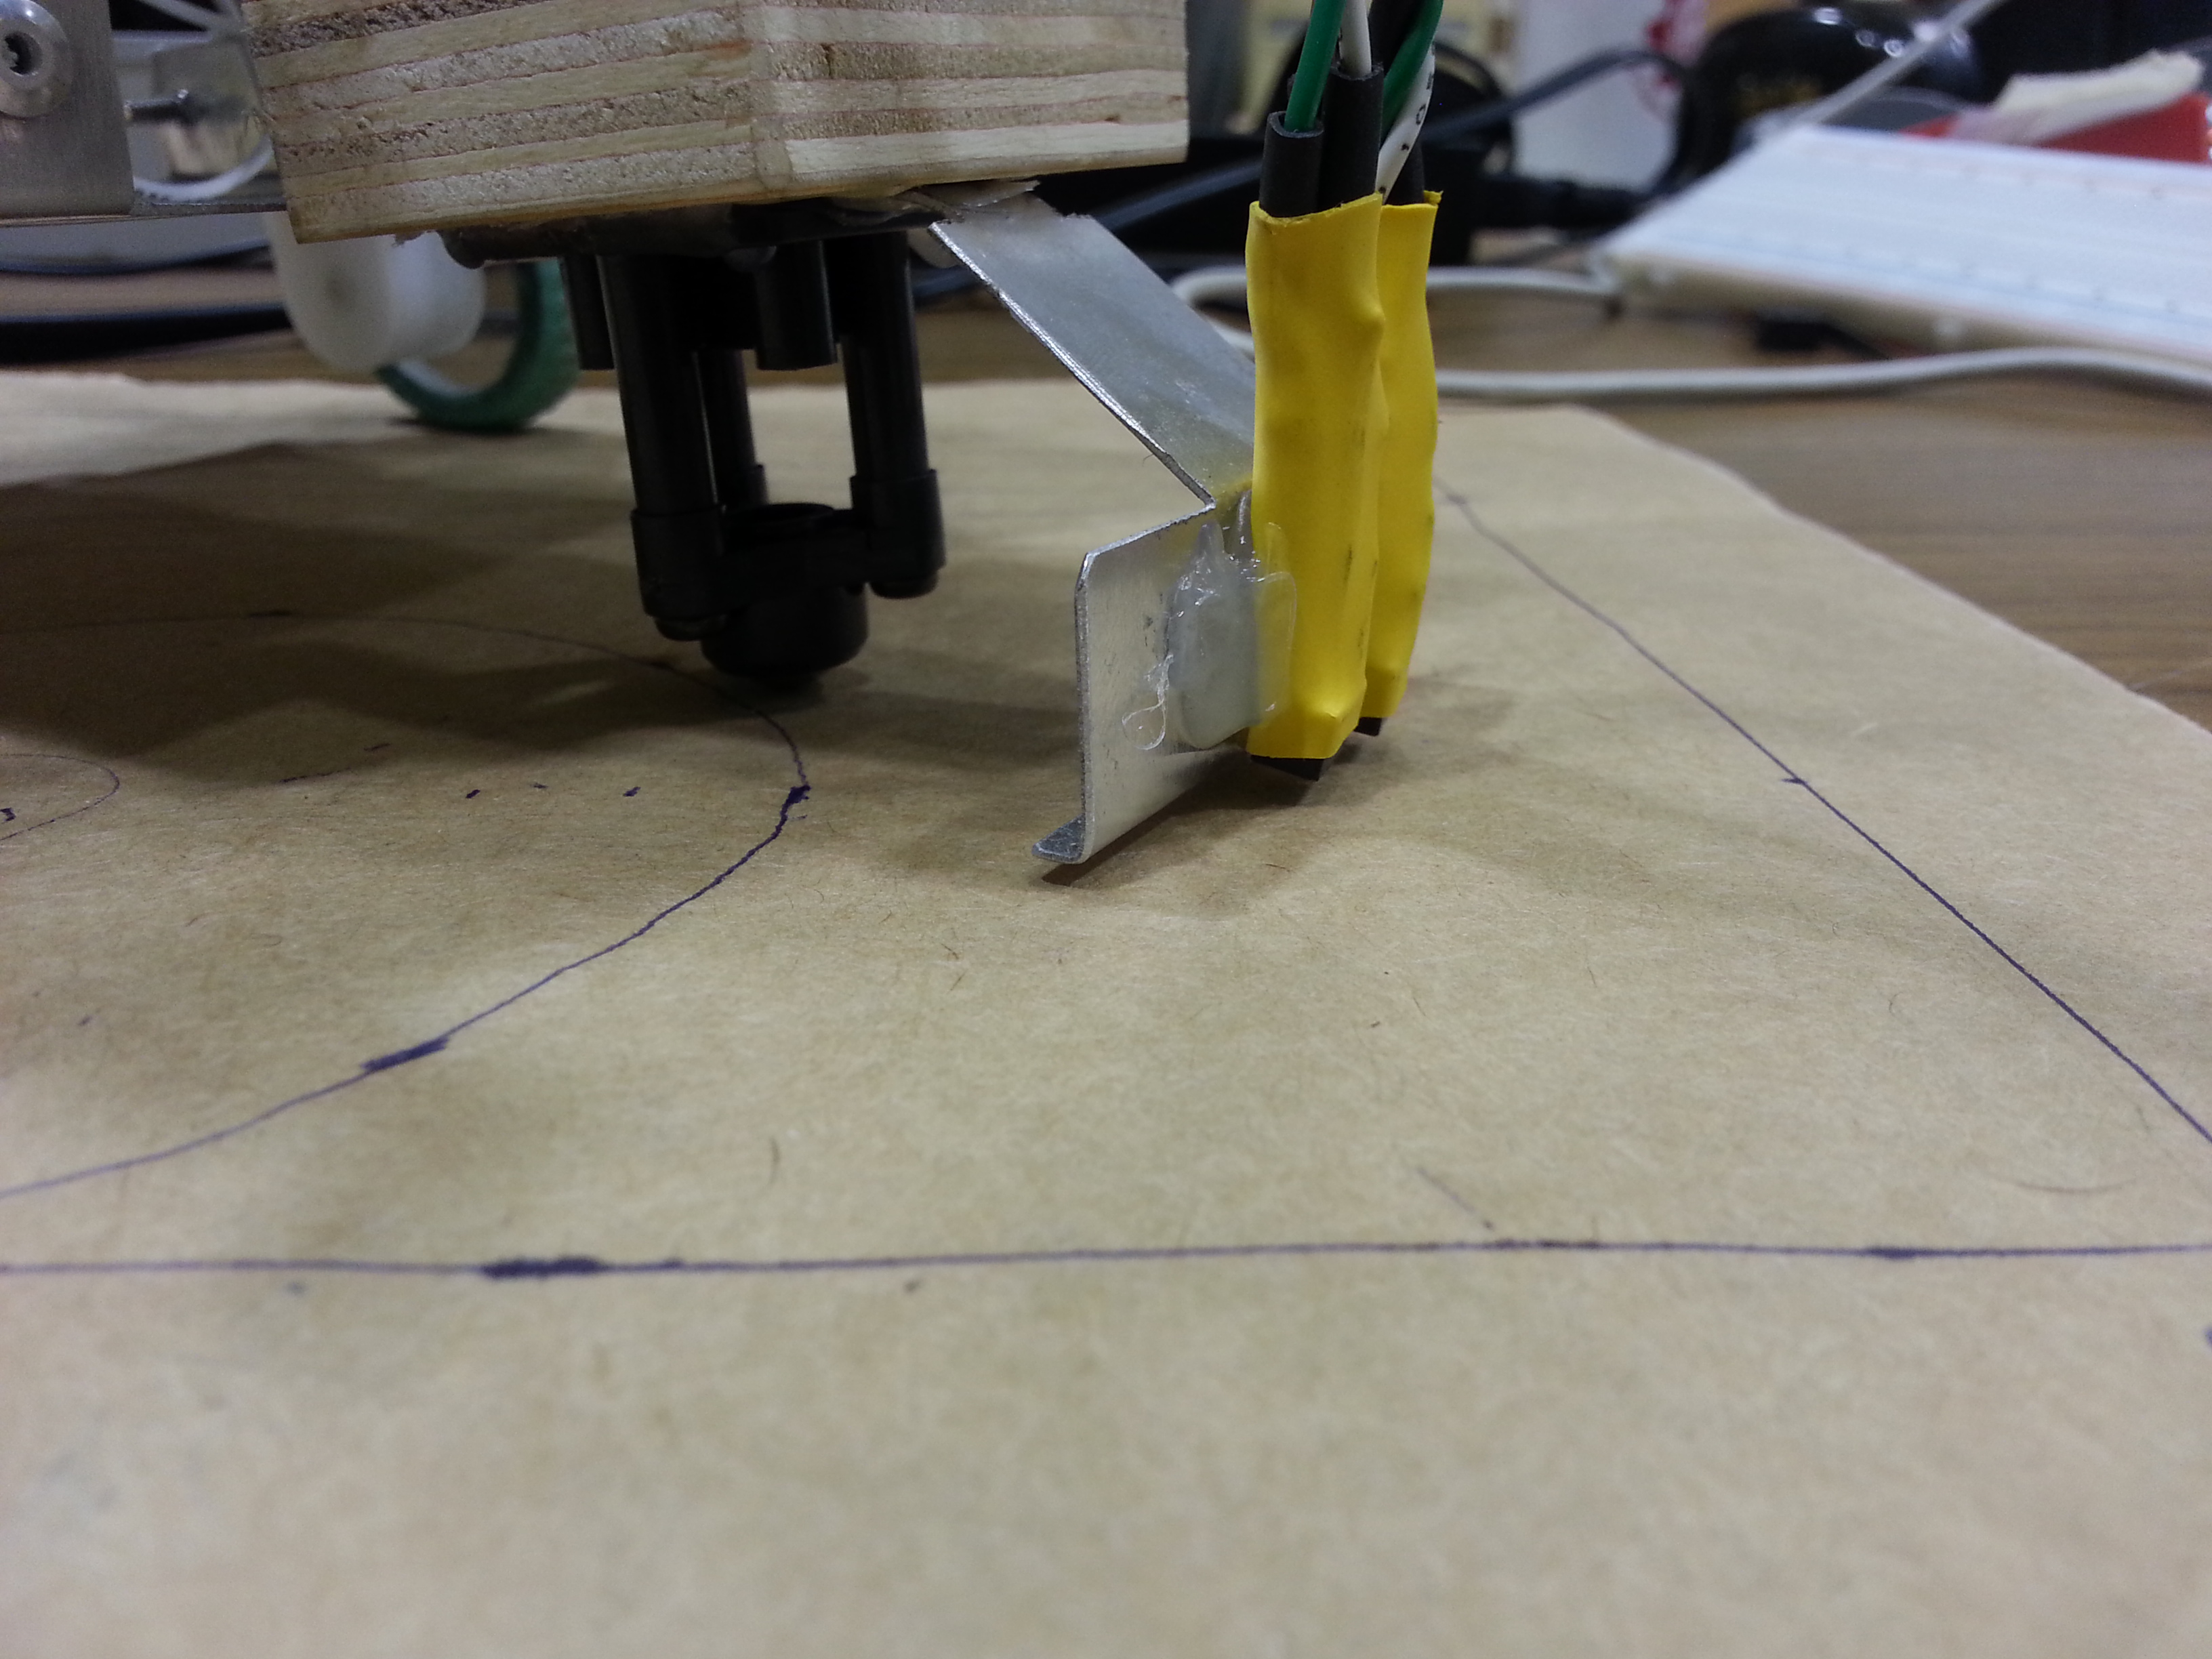
\includegraphics[width=0.7\textwidth]{Figures/reflectance_sensors.jpg}
		\caption{The metal sensor bracket can be bent to adjust the sensors' position.}
	\end{figure}

\subsection{Using the Tuning Menu}

	Once booted, the TINAH board will display several values on the LCD screen. Each value is a tuning parameter that changes the performance of the tape follower. The LCD screen will show one value at a time. To change the displayed value, rotate the upper knob found on the bottom left of the TINAH board, as shown in Figure 3.

	\begin{figure}[h]
	\centering
		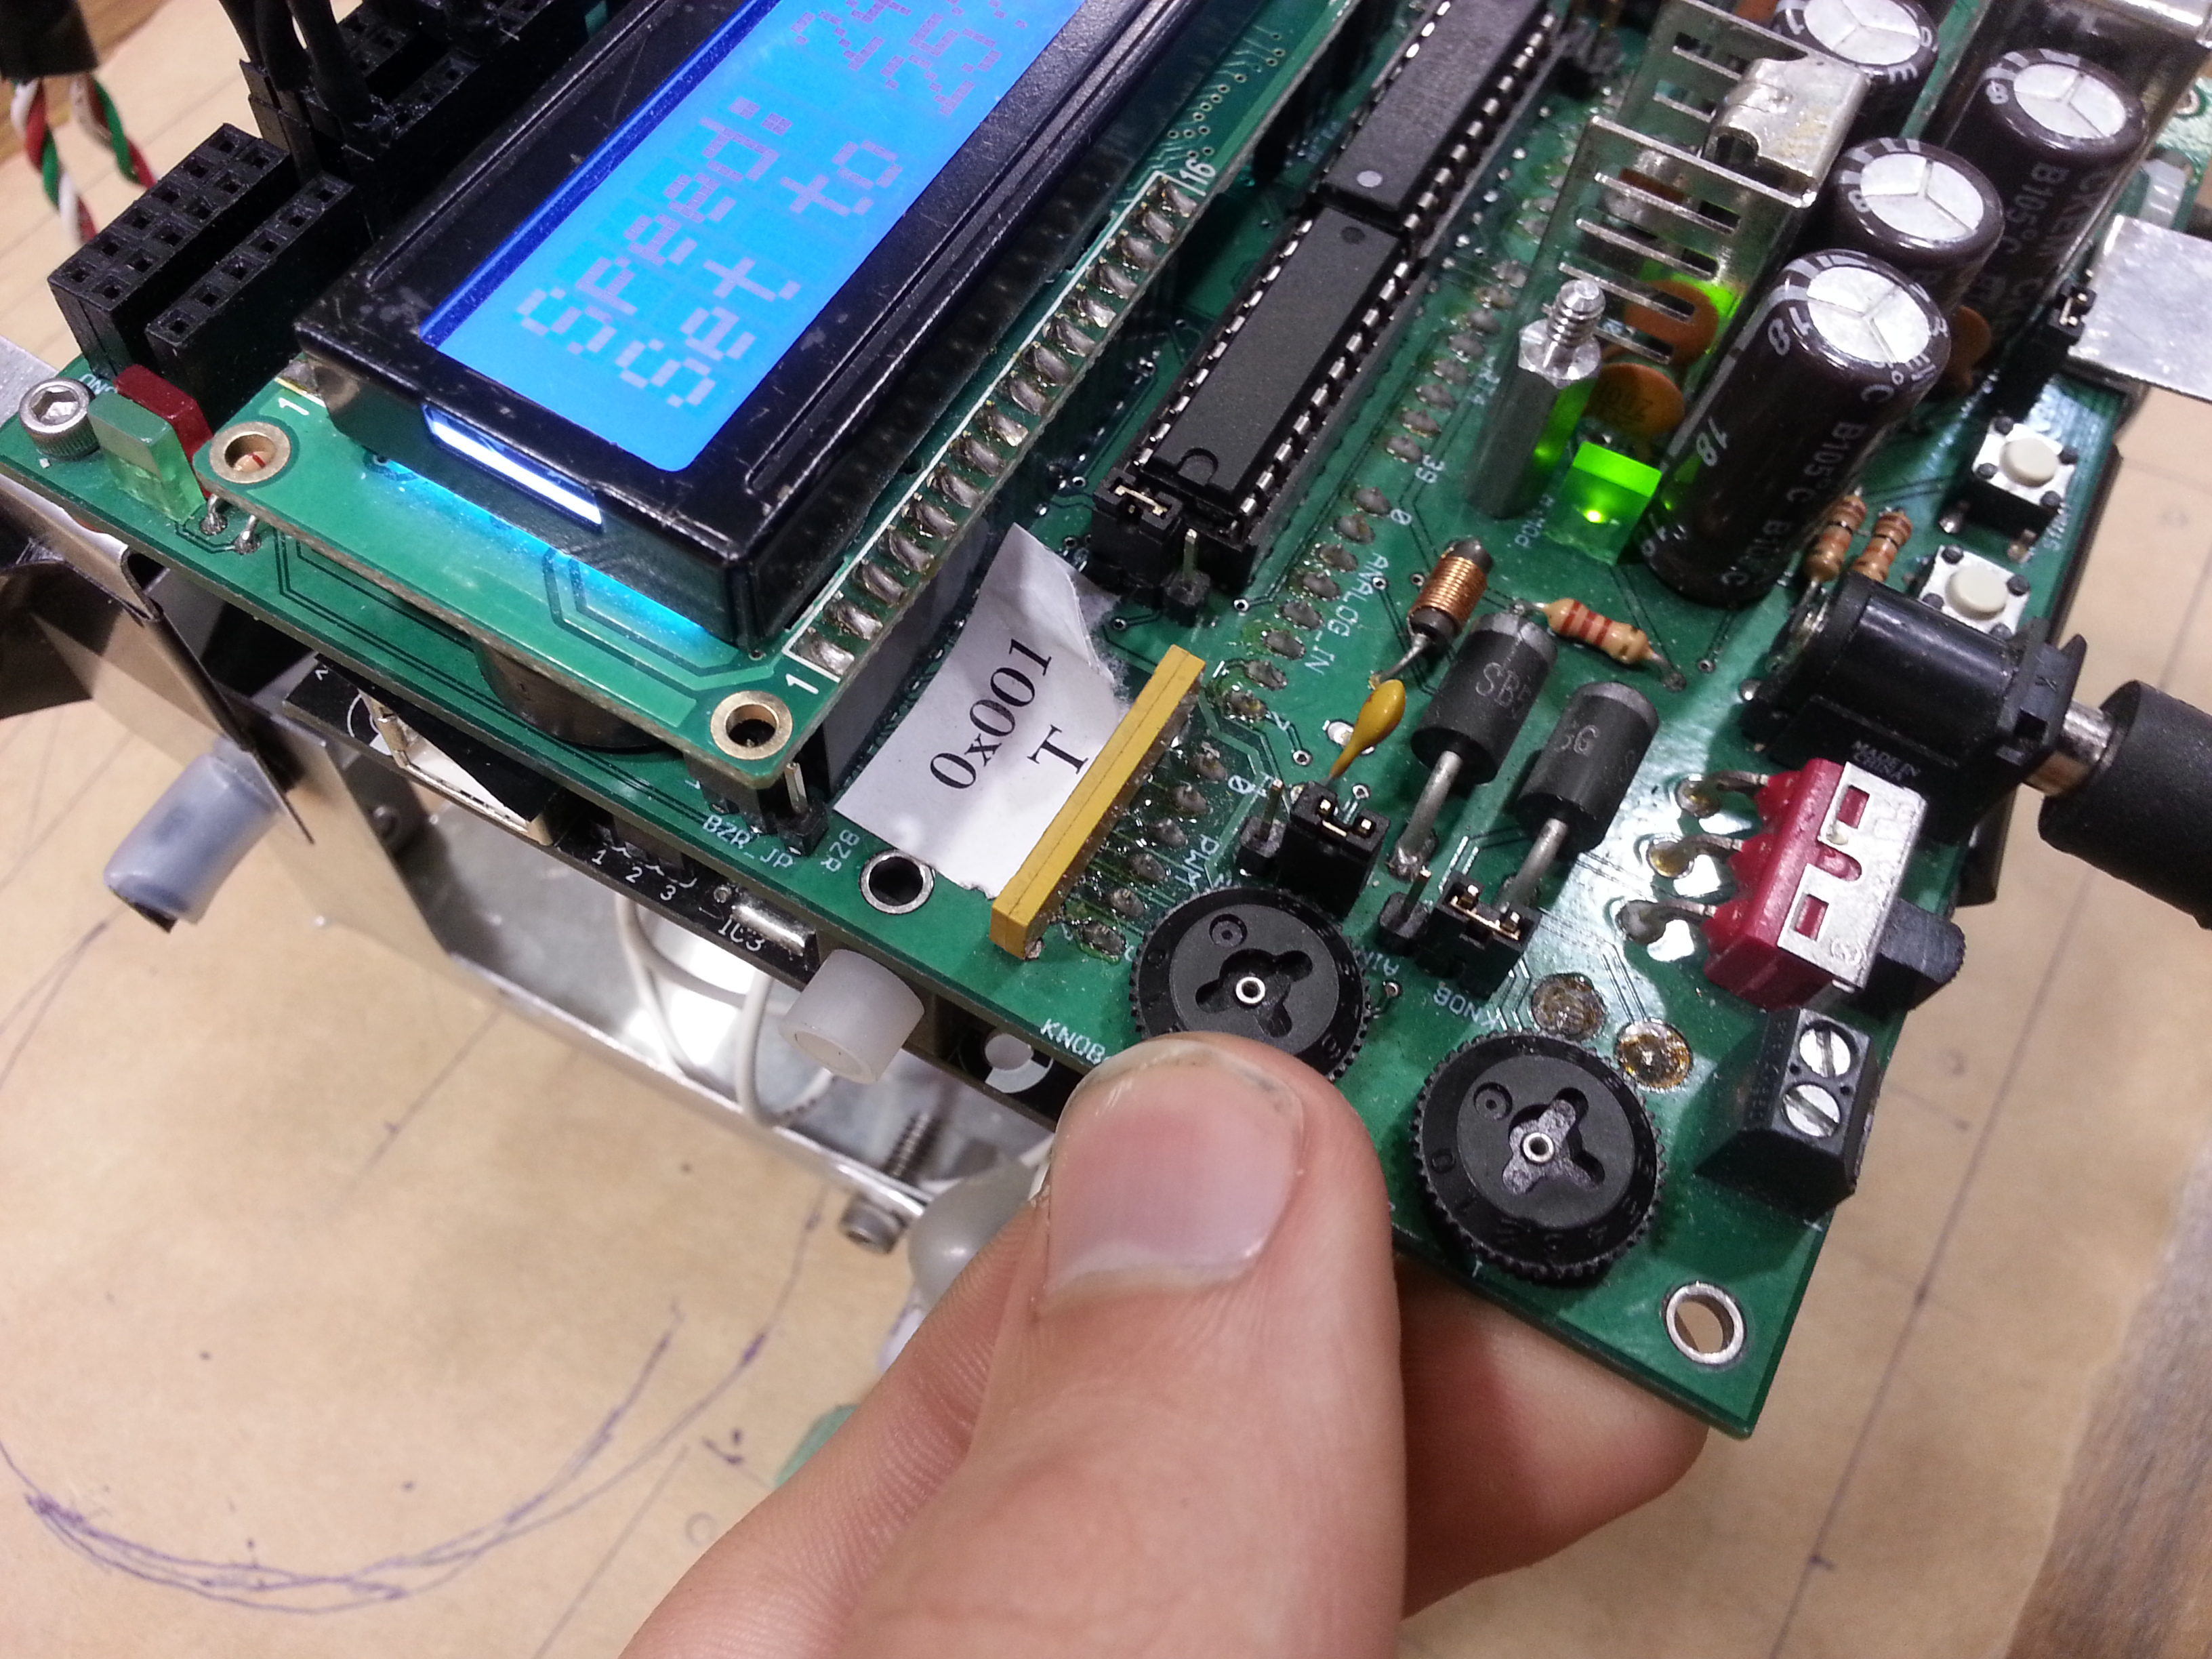
\includegraphics[width=0.7\textwidth]{Figures/knobs.jpg}
		\caption{The upper knob controls the tuning parameter displayed on the LCD screen.}
	\end{figure}

	The value of each tuning parameter can be changed by rotating the lower knob, found on the bottom left of the TINAH board.  The tuning parameters display along the range 0-255.  To confirm a tuning parameter value change, press the left-most button found along the bottom of the TINAH board, as shown in Figure 4. This will save the tuning parameter TINAH's permanent memory, storing its value even when the TINAH is powered off.
	
	\begin{figure}[h]
	\centering
		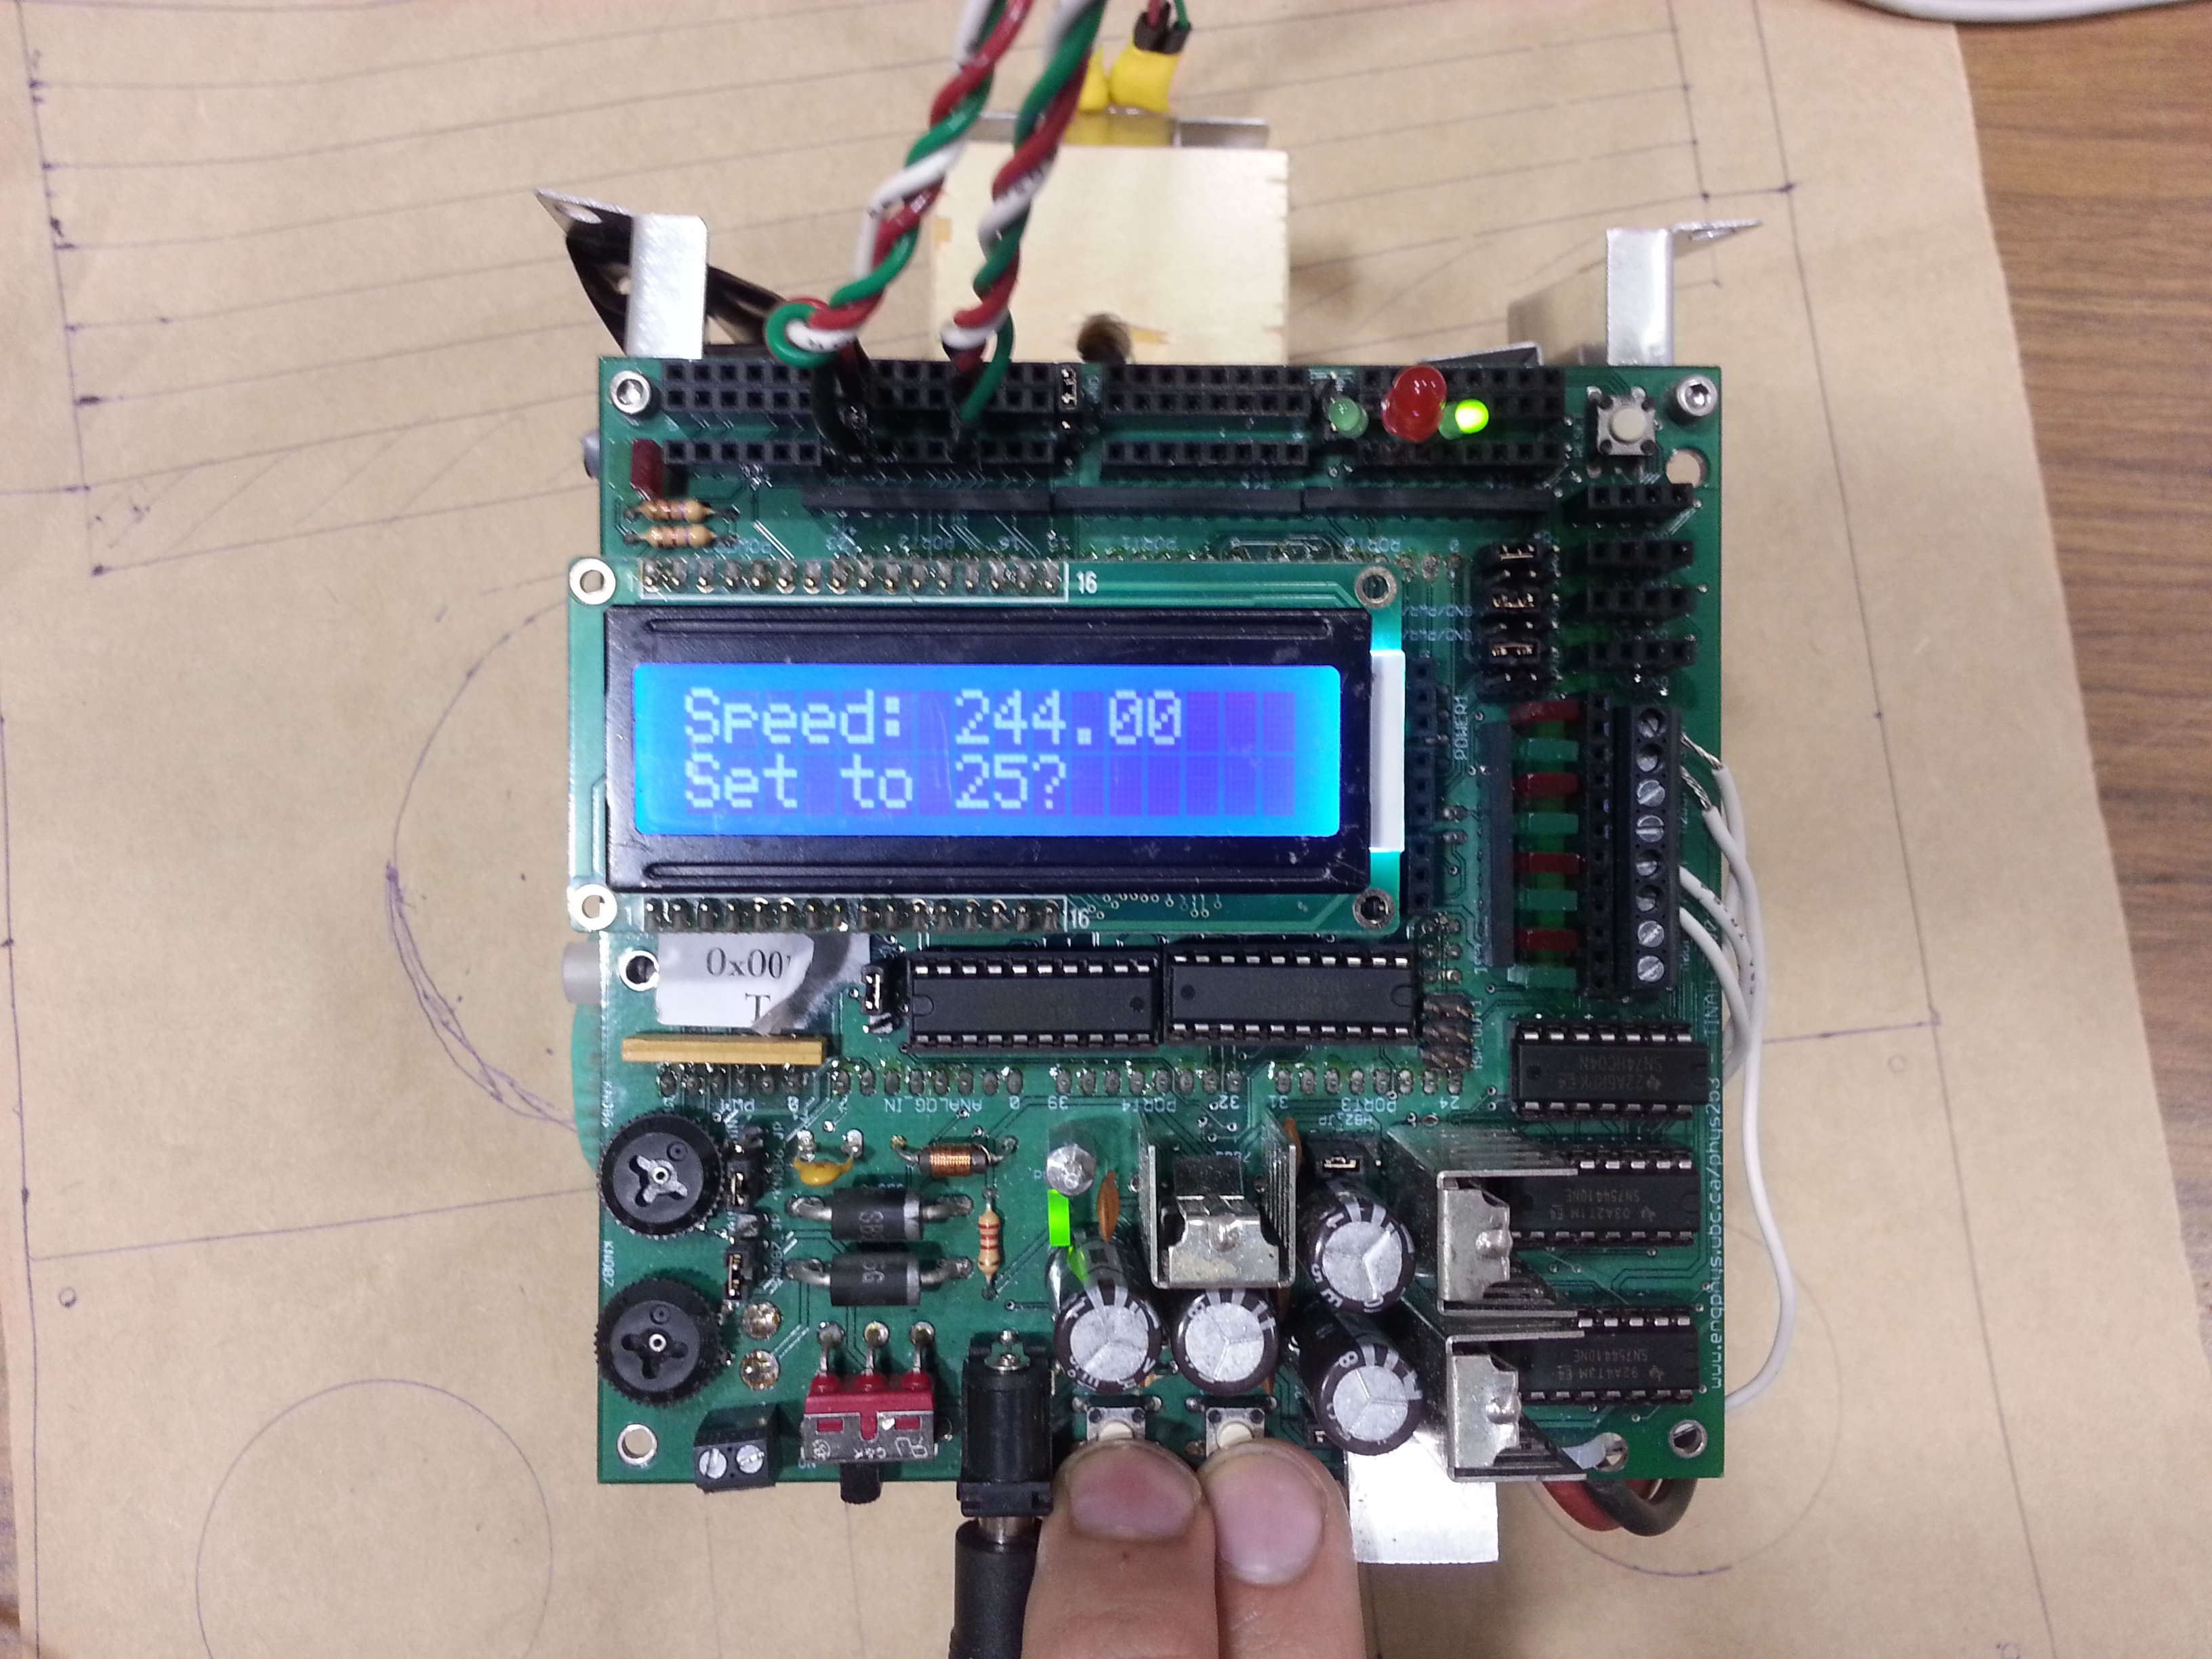
\includegraphics[width=0.7\textwidth]{Figures/buttons.jpg}
		\caption{The left and right buttons allow the user to confirm changes and exit the tuning menu, respectively.}
	\end{figure}
	
	The tuning parameters are each explained in the following list.
	
	\begin{itemize}
	
		\item ``P Gain'' stands for Proportional Gain. Increasing this value will make the tape follower compensate more sharply when veering off course. Decreasing this value will make the tape follower less sensitive to error.
		
		\item ``D Gain'' stands for Derivative Gain. Higher values of derivative gain will increase the rate at which the robot reacts to changing errors in tape following. A value too large will cause the robot to zigzag erratically.
		
		\item ``Speed'' represents the overall speed of the tape follower. Large speed values may be unstable and the tape follower may be too slow to react to error.
		
		\item ``Thresh'' stands for Threshold, this represents the minimum amount of reflected light that the robot will consider to be tape. If this value is too low, everything will be considered tape. If it is too high, then nothing will be considered tape and the robot will be unable to navigate. It is good practice to set the threshold about 10 units higher than the ambient white floor.
	 
	\end{itemize}	

\subsection{Tuning}
	
	Tuning involves adjusting the parameters in a specific order, observing the robot's behavior to determine the necessary changes.
	
	\begin{enumerate}
	
	 	\item Begin by setting proportional gain to about 128, derivative gain to 0, speed to around 50, and the threshold to about 10 above the values sensed when the robot is off of the tape.  The current sensor values are displayed on the LCD screen when setting the threshold parameter.
	 	
	 	\item Switch the robot to its line following mode by pressing the right-most button along the bottom of the TINAH board.  Observe its behavior.  Continue to increase its proportional gain until it begins to zigzag noticeably when following straight tape lines.
	 	
	 	\item Set derivative gain to 128 and observe the robot's line following on both straight and curved tape lines.  If the robot is still zigzagging, increase the derivative gain.
	 	
	 	\item Increase the speed by about 50.  If the robot still line follows well, try further increasing the speed.  If the robot's turns cannot ``keep up'' with the tape line, increase the proportional gain.  If more zigzagging occurs, increase the derivative gain or adjust the proportional gain down slightly.

	\end{enumerate}

\end{adjustwidth}	

\section{Conclusion}

The robot has now been tuned to follow tape quickly and accurately.  The robot's sensors and TINAH board were setup and the PID tuning menu was used to adjust the tuning parameters.  If the robot is not behaving as expected, slowing down or seeming to ignore the tape, double check all electrical connections and the current charge of the battery.

\end{document}